\documentclass[a4paper]{article}
\usepackage{graphicx}
\usepackage[margin = 1in]{geometry}
\usepackage{ragged2e}
\usepackage[hidelinks, colorlinks = true, citecolor = black, linkcolor = blue]{hyperref}
\usepackage{parskip}
\usepackage{cite}
\usepackage{caption}
\usepackage{subcaption}
\usepackage{cellspace}
\usepackage{makecell}
\usepackage{mwe}
\setlength\cellspacetoplimit{4pt}
\setlength\cellspacebottomlimit{4pt}
\usepackage{caption} 
\usepackage{pgfplots}
\usepackage{amsmath}
\usepackage{tikz}
\usepackage{pdfpages}
\newcommand{\inv}{^{\raisebox{.2ex}{$\scriptscriptstyle-1$}}}
\newcommand{\unit}[1]{~\mathrm{#1}}
\captionsetup[table]{skip=10pt}
\renewcommand{\arraystretch}{1.5}


\usepackage{tikz}
\usetikzlibrary{shapes,arrows,positioning,fit,backgrounds,calc}
\usepackage{pgfplots}
\pgfplotsset{compat=1.16}
\pgfplotsset{ignore zero/.style={%
  #1ticklabel={\ifdim\tick pt=0pt \else\pgfmathprintnumber{\tick}\fi}
}}
\usepackage{pgf}
\begin{document}

\section{Introduction}
A potentiometer is an electrical component that functions both as a variable resistor and as a voltage divider.
It allows for the precise adjustment of electrical resistance and the control of output voltage in a circuit. 
The aim of the experiments detailed in this report is to analyze the behavior and characteristics of the potentiometer
in various circuit configurations.
\section{Background/Theory}
A potentiometer is a resistor that has three terminals. Two of the terminals
constitute the full resistance value, while the third one is a sliding contact.
Figure 1 displays the different contacts of the potentiometer.
\begin{figure}[!ht]
    \centering
    \begin{minipage}{0.4\textwidth}
        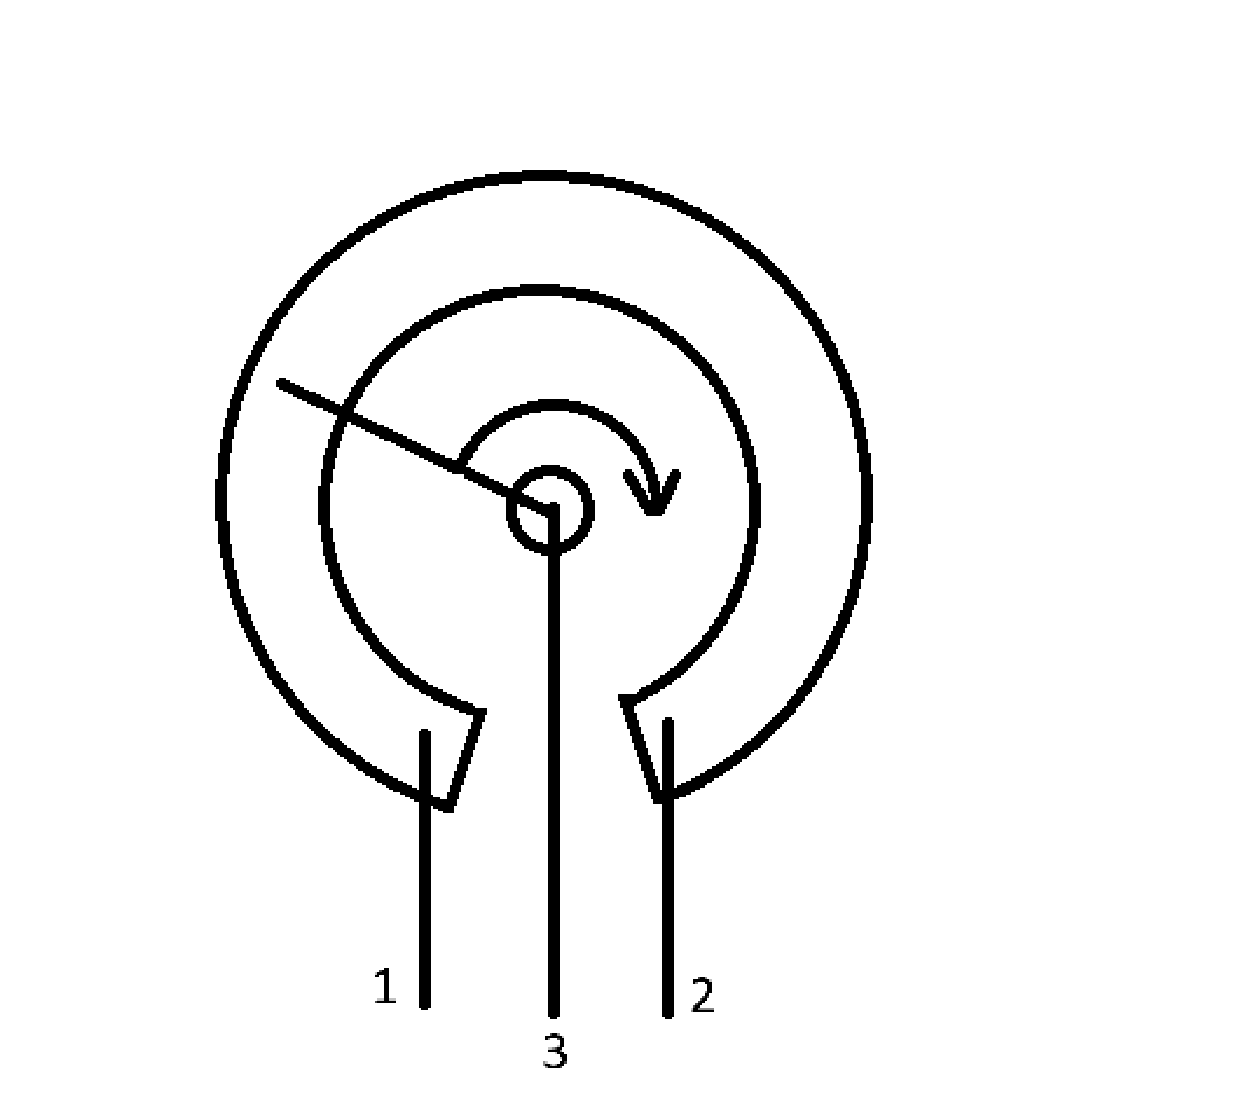
\includegraphics[width = \textwidth]{potterminals.png}
       \label{fig:1}
        \caption{\centering Drawing of a potentiometer with labeled terminals}    
    \end{minipage}
\end{figure}

The resistance between terminals 1 and 2 is constant, while the resistance
between 1 and 3 is determined by equation 1:
\begin{equation}
    R_{13} = kR
\end{equation}
%ref

Since the potentiometer can be used as a voltage divider, the value of the
potential difference between terminals 1 and 3 will be determined using equation 2:
\begin{equation}
    V_{13} = k V_{tot}
\end{equation} 

When adding a load resistor in parallel to terminals 1 and 3, the voltage across
them can be calculated using equation:
%refr
\begin{equation}
    V_{13} = \frac{kR_{13}}{R_{13}+k(1-k)R_p} V
\end{equation}
\section{Methods \& Materials}
All circuits in the experiments were assembled using the provided connection boards. 
The electrical measurements, including voltage and current, were performed using the AM-520 
HVAC multimeter for precision. 
A 10-turn potentiometer with a total resistance of $1 k~\Omega$ and a resolution of $\Delta k = 0.001$ 
was used to vary resistance and control output voltage. 
The power supply consisted of two 1.5V batteries connected in series. 
Fixed resistors of $1 ~k\Omega$  and $510 ~k\Omega$  were utilized as load resistors, 
along with a decade resistor to provide 
adjustable resistance for certain measurements.


\newpage
\subsection{Experimental Set-Up unloaded potentiometer}
An unloaded potentiometer circuit comprises a voltage source and a potentiometer.
Measurementeasurements are taken for both the voltage supplied by the power source
and the potential difference established between terminals 1 and 3. 

In the unloaded potentiometer circuit, measurements are conducted incrementally by varying the parameter 
k from 1 to 0.1. 

Figures 2(a) and 2(b) display both
the electrical diagram, and a picture of the physical set-up of the circuit.

\begin{figure}[!h]
    \centering
    \begin{subfigure}{.5\textwidth}
        \centering
        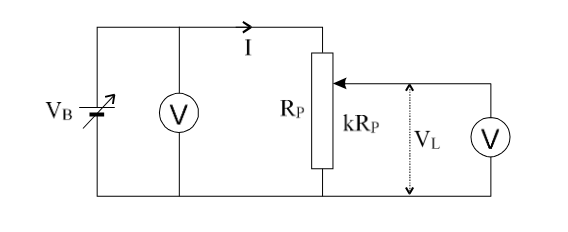
\includegraphics[width=0.8\linewidth]{Unloaded pot circuit.png}
        \label{fig:2a}
        \caption{Circuit diagram of unloaded potentiometer circuit(refr)}   
    \end{subfigure}%
    \begin{subfigure}{.5\textwidth}
        \centering
        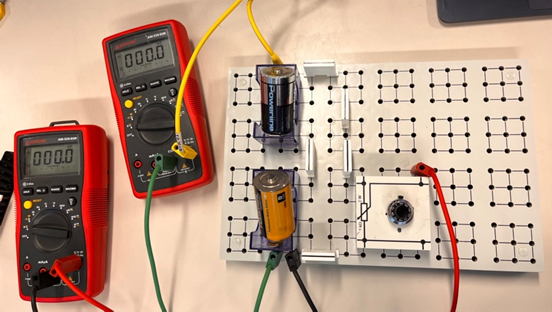
\includegraphics[width = 0.8\linewidth]{unloaded pot picture.png}
        \label{fig2:b}
        \caption{Picture of the unloaded potentiometer circuit}
    \end{subfigure}
    \caption{Electrical schema and physical set-up of the unloaded potentiometer circuit}
\end{figure}
\subsection{Experimental Set-Up with fixed resistor}
The experimental set-up for the second experiment mirrors that of the first, 
with the key distinction being the addition of a load resistor connected in parallel across terminals 1 and 3.
Specifically, a 510 $\Omega$ resistor and a 1 k$\Omega$ resistor are incorporated to introduce varying load conditions.

Figures 3(a) and 3(b) display both the electrical diagram and a picture of the
physical set-up of the circuit.
\begin{figure}[!ht]
    \centering
    \begin{subfigure}{0.5\textwidth}
        \centering
        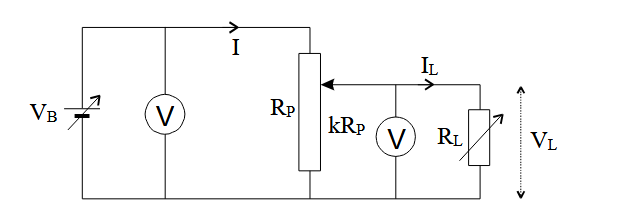
\includegraphics[width = \linewidth]{loaded pot fixed circuit.png}
        \label{fig:3a}
        \caption{Circuit diagram of the loaded \\potentiometer circuit}
    \end{subfigure}%
    \begin{subfigure}{0.5\textwidth}
        \centering
        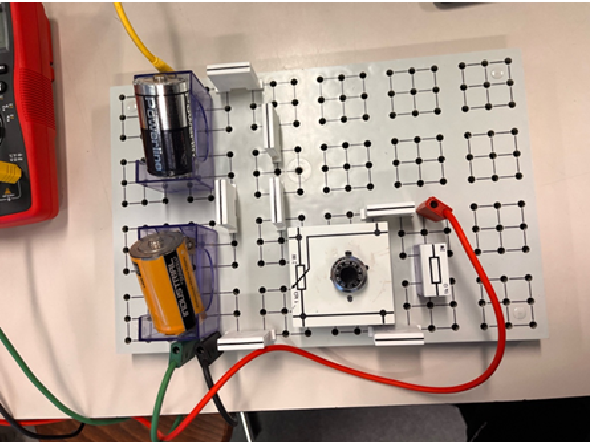
\includegraphics[width = 0.8\linewidth]{loaded pot fixed pic.png}
        \label{fig:3b}
        \caption{Picture of the loaded potentiometer circuit with fixed resistance}        
    \end{subfigure}
    \caption{Electrical schema and physical set-up of the loaded potentiometer with fixed resistance}
\end{figure}
\newpage
\subsection{Experimental Set-Up with fixed load current}
The set-up for the third experiment omits the voltmeter measuring the power
source, replacing it with an ammeter in line with the load resistor. The load
resistor being used becomes a decade resistor.

The experimental flow is also changed, as now with a change in the k-value, the
decade resistor is adjusted in order for the current load to remain the same,
then the resistance of the decade resistor, and the voltage drop is measured.

Figures 4(a), and 4(b) display the circuit diagram and picture of this
experiment.

\begin{figure}[!ht]
    \centering
    \begin{subfigure}{.5\textwidth}
        \centering
        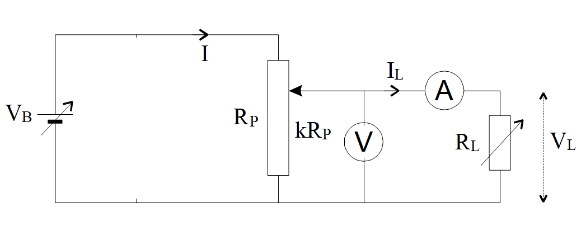
\includegraphics[width = 0.8\linewidth]{fixed current circuit.png}
        \label{fig:4a}
        \caption{Circuit diagram of the constant current load circuit(refr)}
        
    \end{subfigure}%
    \begin{subfigure}{.5\textwidth}
        \centering
        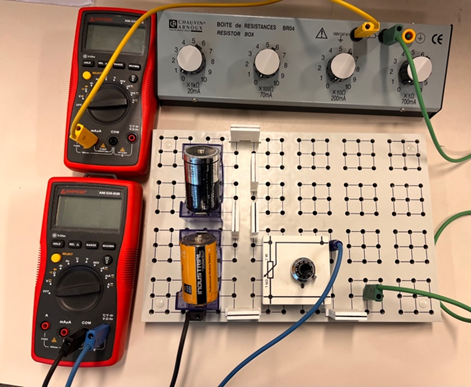
\includegraphics[width = 0.8\linewidth]{fixed currrent picture.png}
        \label{fig:4b}
        \caption{Picture of the constant current load circuit}
    \end{subfigure}
    \caption{Electrical diagram and physical set-up of the constant current load circuit}
\end{figure}
\section{The Unloaded Potentiometer}
\subsection{Measurement Results}
Table 1 presents the measured voltage values corresponding to different values of 
the parameter k, alongside the theoretical voltage values and 
the associated measurement error for the unloaded potentiometer circuit.
\begin{table}[!ht]
    \centering
    \label{tab:1}
    \caption{Measured and expected voltage in terms of the parameter k of the potentiometer}
    \begin{tabular}{|c c c c|} 
    \hline
    $k$ & \makecell{$V_{unloaded}$ \\ (V)} & \makecell{$\Delta V_{unloaded}$ \\ (V)} &
    \makecell{$V_{expected}$ \\ (V)}  \\ 
    \hline
    0.1                                       & 0.302      &  0.009          & 0.296      \\
    0.2                                       & 0.594      &   0.009         & 0.592      \\
    0.3                                       & 0.89       &   0.017         & 0.888      \\
    0.4                                       & 1.184      &  0.014          & 1.184      \\
    0.5                                       & 1.481      &  0.013          & 1.480      \\
    0.6                                       & 1.776      &  0.021          & 1.775      \\
    0.7                                       & 2.076      &  0.023          & 2.071      \\
    0.8                                       & 2.365      &  0.024          & 2.367      \\
    0.9                                       & 2.663      &  0.025          & 2.663      \\
    1.0                                       & 2.957      &  0.031          & 2.959      \\
    \hline
    \end{tabular}
    \end{table}
\newpage
\subsection{Graphs}
Figure 5 illustrates the relationship between the measured voltage and the parameter 
k in the unloaded potentiometer circuit.
\begin{figure}[!ht]
    \centering
    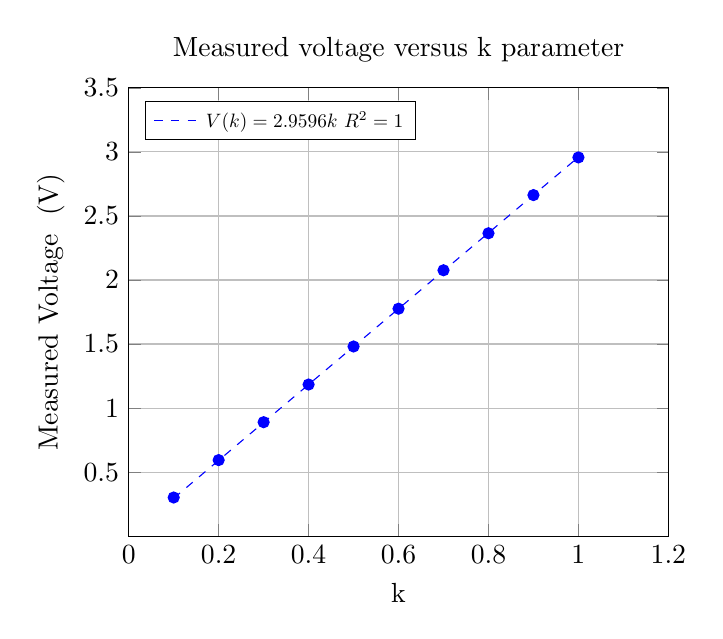
\begin{tikzpicture}
        \begin{axis}[
            title = {Measured voltage versus k parameter},
            xlabel = {k},
            ylabel = {Measured Voltage $ \unit{(V)}$},
            xmin = 0, xmax = 1.2,
            ymin = 0, ymax = 3.5,
            xtick = {0, 0.2, 0.4, 0.6, 0.8, 1.0, 1.2},
            ytick = {0, 0.5, 1, 1.5, 2, 2.5, 3, 3.5},
            ymajorgrids = true,
            xmajorgrids = true,
            legend pos = north west,
            legend style={nodes={scale=0.7}},
            domain = 0.1:1,
            ignore zero = y
        ]
        
        \addplot[blue, samples = 100, dashed]{2.9596*x};
        
        \addplot[only marks, color = blue] coordinates {
            (0.1, 0.302)
            (0.2, 0.594)
            (0.3, 0.89)
            (0.4, 1.184)
            (0.5, 1.481)
            (0.6, 1.776)
            (0.7, 2.076)
            (0.8, 2.365)
            (0.9, 2.663)
            (1.0, 2.957)
        };
        
        \legend{$V(k) = 2.9596k$ $R^2 = 1$}
        
        \end{axis}
    \end{tikzpicture}
    \caption{Measured voltage (V) drop in terms of the k parameter}
    \label{fig:3}
\end{figure}

\subsection{Discussion}
The main goal of this experiment was to determine the effect of changing the
k-value of the potentiometer on the voltage load of the varying resistance. When
looking at the graphical representation of these values seen on figure 3, we see
a linear relationship between the k-value and the voltage drop on the
potentiometer.

Analyzing the difference between the measured and expected
voltage, we see that the measured values are accurate, as the difference between
them and the expected values falls within the measurement error. 
\newpage
\section{Potentiometer loaded with fixed resistor}
\subsection{Measurement results}
Table 2 presents the measurements for k,
including the unloaded potentiometer value and the values corresponding to both loads,
$1 k\Omega$ as load 1 and $510~\Omega$ as load 2.
The table provides both the measured $V_{L1}$ and $V_{L2}$ values, and theoretical values $V_{L1t}$ and $V_{L2t}$, 
along with the calculated percent deviations $PD_1$ and $PD_2$.
\begin{table}[!ht]
    \centering
    \label{tab:2}
    \caption{Measured and theoretical voltage for $1 k\Omega$ and $510\Omega$
    load values in terms of k}
    \begin{tabular}{|c c c c c c c c|} 
    \hline
    $k$ & \makecell{$V_{unloaded}$\\ (V)} & \makecell{$V_{L1}$\\ (V)} & 
    \makecell{$V_{L1t}$\\ (V)} & \makecell{$PD_{1}$\\ (\%)}  & \makecell{$V_{L2}$\\ (V)} &
    \makecell{$V_{L2t}$\\ (V)}
    & \makecell{$PD_2$ \\ (\%)}   \\ 
    \hline
    0.1     & 2.959    & 0.274  & 0.156                & 75.85 & 0.253  & 0.111                & 56.02  \\
    0.2     & 2.959    & 0.514  & 0.329                & 56.27 & 0.451  & 0.239                & 46.98  \\
    0.3     & 2.959    & 0.739  & 0.522                & 41.46 & 0.628  & 0.388                & 38.28  \\
    0.4     & 2.959    & 0.957  & 0.740                & 29.32 & 0.809  & 0.562                & 30.53  \\
    0.5     & 2.959    & 1.184  & 0.987                & 20.00 & 0.993  & 0.770                & 22.47  \\
    0.6     & 2.959    & 1.433  & 1.269                & 12.97 & 1.21   & 1.022                & 15.55  \\
    0.7     & 2.959    & 1.717  & 1.594                & 7.74  & 1.47   & 1.334                & 9.27   \\
    0.8     & 2.959    & 2.039  & 1.973                & 3.35  & 1.801  & 1.730                & 3.97   \\
    0.9     & 2.959    & 2.448  & 2.421                & 1.11  & 2.268  & 2.249                & 0.86   \\
    1.0       & 2.959    & 2.952  & 2.959                & 0.24  & 2.948  & 2.959                & 0.37   \\
    \hline
    \end{tabular}
    \end{table}
\subsection{Graphs}
Figure 6 illustrates the relationship between the voltage across the load resistor
and the parameter 
k, comparing the experimental results with the 
corresponding theoretical values. 
Additionally, it presents the voltage drop across the unloaded potentiometer for reference.
\begin{figure}[!ht]
    \centering
    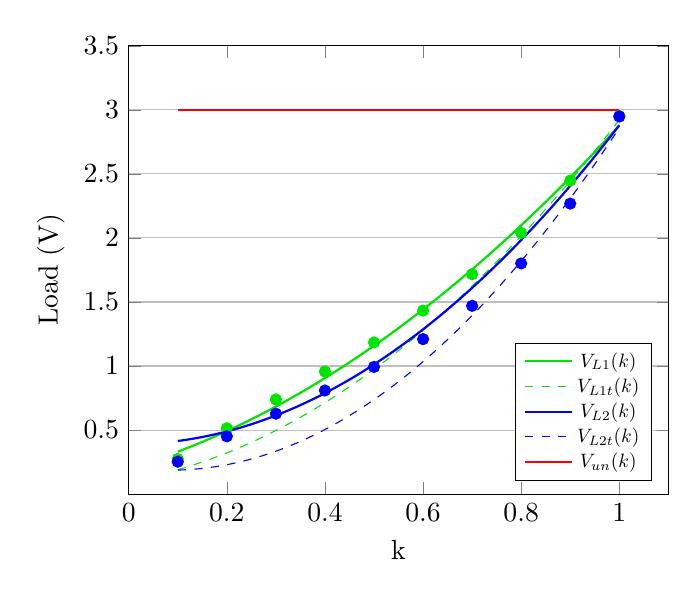
\begin{tikzpicture}
        \begin{axis}[legend pos = south east, legend style={nodes={scale=0.7}}, ymajorgrids = true, domain = 0.1:1, xmin = 0, xlabel = k, xtick = {0, 0.2, 0.4, 0.6, 0.8, 1.0, 1.2}, ymin = 0, ymax = 3.5, ytick = {0, 0.5, 1, 1.5, 2, 2.5, 3, 3.5}, ylabel = Load$ \unit{(V)}$, ignore zero = y, ]
        
        \addplot[black!10!green, thick, samples = 100]{1.52*(x^2) + 1.157*x +0.2};
        \addplot  [only marks, color = black!10!green, forget plot] coordinates {
            (0.1,	0.274)
            (0.2,	0.514)
            (0.3,	0.739)
            (0.4,	0.957)
            (0.5,	1.184)
            (0.6,	1.433)
            (0.7,	1.717)
            (0.8,	2.039)
            (0.9,	2.448)
            (1.0,	2.952)

            
        };
         
        \addplot[black!10!green, thin, samples = 100, dashed]{2.15*(x^2) + 0.67 * x +
        0.102};
        \addplot[blue, thick, samples=100]{2.49*(x^2) + 0.39};
        \addplot  [only marks, color = blue, forget plot] coordinates {
            (0.1,	0.253)
            (0.2,	0.451)
            (0.3,	0.628)
            (0.4,	0.809)
            (0.5,	0.993)
            (0.6,	1.21)
            (0.7,	1.47)
            (0.8,	1.801)
            (0.9,	2.268)
            (1.0,	2.948)
            

            
        };
        \addplot[blue, thin, samples=100, dashed]{3.19*(x^2) - 0.54 * x + 0.21};
        \addplot[red, thick, samples = 100]{3};
        \legend{$V_{L1}(k)$, $V_{L1t}(k)$,$V_{L2}(k)$, $V_{L2t}(k)$,$V_{un}(k)$ }
        \end{axis}
    \end{tikzpicture}
    \label{fig:5}
    \caption{Loads in terms of k}
\end{figure}
\par 
Furthermore, figure 7 displays the relationship between percent deviation
and the k parameter
\begin{figure}
    \centering
    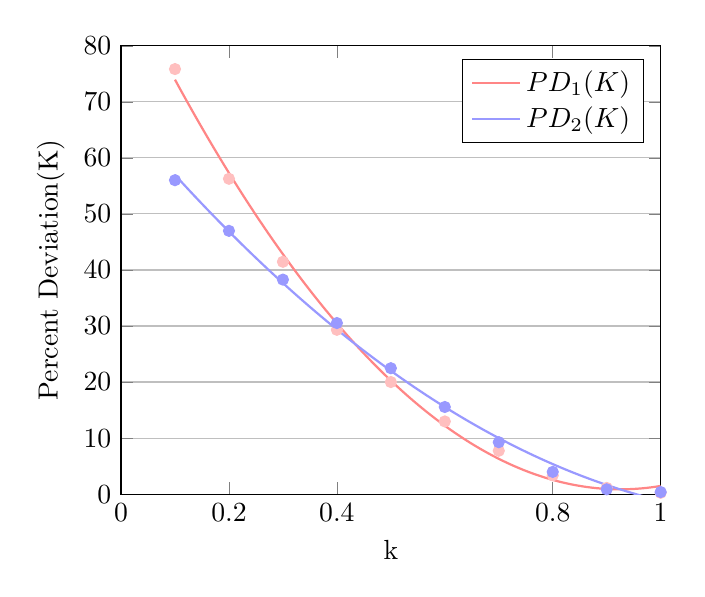
\begin{tikzpicture}
        \begin{axis}[legend pos = north east, legend style={nodes={scale=1}},
        ymajorgrids = true, domain = 0.1:1, xmin = 0, xmax = 1, ymin = 0, ymax =
        80, xlabel = k, xtick = {0, 0.2, 0.4, 0.8, 1}, ytick = {0, 10, 20, 30,
        40, 50, 60, 70, 80}, ylabel = Percent Deviation(K)]
        \addplot[red!30!pink, thick, samples = 100]{107.36*(x^2) - 198.65*x +92.75};
        \addplot[only marks, color = pink, forget plot] 
        coordinates {
            (0.1,	75.85)
            (0.2,	56.27)
            (0.3,	41.46)
            (0.4,	29.32)
            (0.5,	20.00)
            (0.6,	12.97)
            (0.7,	7.74)
            (0.8,	3.35)
            (0.9,	1.11)
            (1.0,	0.24)
             
        };
        \addplot[white!60!blue, thick, samples = 100]{45.56*(x^2) - 114.72*x + 67.98};
        \addplot[only marks, color = white!60!blue, forget plot] 
        coordinates{    
        (0.1,	56.02)
        (0.2,	46.98)
        (0.3,	38.28)
        (0.4,	30.53)
        (0.5,	22.47)
        (0.6,	15.55)
        (0.7,	9.27)
        (0.8,	3.97)
        (0.9,	0.86)
        (1.0,	0.37)
        };
        \legend{$PD_ 1(K)$,$PD_2(K)$}
        \end{axis}
    \end{tikzpicture}
    \label{fig:6}
    \caption{Percent deviation in terms of k}
\end{figure}
\subsection{Calculations}
\subsection{Discussion}
\end{document}